%-----------------------------------------------------------------------
%
%   UFRJ  - Universidade Federal do Rio de Janeiro
%   COPPE - Coordena��o dos Programas de P�s-gradua��o em Engenharia
%   PEE   - Programa de Engenharia El�trica
%
%   COE-835  Controle adaptativo
%
%   Relat�rio da simula��o
%                                                         Ramon R. Costa
%                                                         05/out/09, Rio
%-----------------------------------------------------------------------
\documentclass[11pt,a4paper]{article}
\usepackage[latin1]{inputenc} %pacote para utilizar palavras acentuadas
\usepackage{amsmath,amssymb}  %pacotes do AMS
\usepackage{latexsym}         %pacote para incluir s�mbolos (ex.\Box)
\usepackage{fancybox,fancyhdr}%pacote com frescuras
\usepackage{graphicx}         %pacote para incluir figuras tipo eps
\usepackage[portuguese]{babel}
\usepackage{xcolor}
\usepackage{float} 
\usepackage{epstopdf}
\usepackage[inline]{enumitem}
\usepackage[a4paper]{hyperref}% Make sure it comes last of your loaded packages
\hypersetup{
  verbose,
  plainpages=false,
  bookmarks=true,
  colorlinks=true,
  linkcolor=blue
}

%Matlab code in latex 
\usepackage[final]{listings}
\usepackage{color} %red, green, blue, yellow, cyan, magenta, black, white
\definecolor{mygreen}{RGB}{28,172,0}
\definecolor{mylilas}{RGB}{170,55,241}
\lstdefinestyle{myMatlab}
{
language=matlab,frame=single, basicstyle=\small\ttfamily,breaklines=true,%
morekeywords={matlab2tikz}, keywordstyle=\color{blue}, morekeywords=[2]{1}, keywordstyle=[2]{\color{black}}, commentstyle=\color{mygreen}, stringstyle=\color{mylilas}, identifierstyle=\color{black}, showstringspaces=false,%without this there will be a symbol in the places where there is a space
numbers=left, numberstyle={\scriptsize \color{black}},% size of the numbers
numbersep=9pt, % this defines how far the numbers are from the text
% emph=[1]{for,end,break},emphstyle=[1]\color{red}, %some words to emphasise
% emph=[2]{word1,word2}, emphstyle=[2]{style},
}
     
%----------------------------------------------------------------------
%
%   Macros utilizados no LATEX
%                                                       Ramon R. Costa
%                                                       13/out/17, Rio
%----------------------------------------------------------------------
\newcount\m
\newcount\n

\def\twodigits#1{\ifnum #1<10 0\fi \number#1}

\def\hours{\n=\time \divide\n 60
    \m=-\n \multiply\m 60 \advance\m \time
    \twodigits\n:\twodigits\m}

\def\hora{\hours}

\def\fim{
  \medskip
  \begin{center}
    \rule[1mm]{30mm}{0.14mm}$\diamond$\rule[1mm]{30mm}{0.14mm}
  \end{center}
}

%----------------------------------------------------------------------
% A4 paper size & margins
\setlength {\textheight}    {25cm}%
\setlength {\textwidth}     {17.5cm}%
\setlength {\parindent}     {0mm}%
\setlength {\parskip}       {1mm}%
\setlength {\topmargin}     {-14mm}%
\setlength {\oddsidemargin} {-6mm}%
\setlength {\evensidemargin}{-6mm}%
\setlength {\columnsep}     {6mm}%

%----------------------------------------------------------------------
\def\codigo{COE-835}
\def\disciplina{Controle adaptativo}
\def\periodo{3o. período/2017}
\def\professor{Ramon}

\newcommand{\BOX}[1]{
  \framebox{{\color{magenta}\rule[-3mm]{1mm}{9mm}} ~~$\displaystyle
  \begin{aligned} #1 \end{aligned}$~~}\pagestyle{plain}
}

\newcommand{\RED}[1]{\colorbox{white}{\textcolor{red}{#1}}}
%\newcommand{\WoR}[1]{\colorbox{red}{\textcolor{white}{#1}}}
\newcommand{\BLU}[1]{\colorbox{white}{\textcolor{blue}{#1}}}
\newcommand{\GRE}[1]{\colorbox{green}{\textcolor{black}{#1}}}
\newcommand{\HI}[1]{\colorbox{yellow}{\textcolor{black}{#1}}}  %% Highlithed text

\newcommand{\estrela}[1]{
  \def\TXT{\RED{$\bigstar$ }}
  \hspace*{5mm}\TXT \hfill
  \parbox[t]{ \textwidth - \widthof{\TXT} - 5mm}{#1}
  \par
}

\def\Ltwo{\mbox{${\mathcal L}_2$}}
\def\Linf{\mbox{${\mathcal L}_\infty$}}

\newcommand{\sign}{\mbox{sign}}

\newcommand{\equacao}[2]{
  \makebox[40mm][l]{#1 \dotfill}: \quad \parbox[t]{8cm}
	{\begin{equation} \displaystyle
  \begin{aligned}
    #2
  \end{aligned} \end{equation}} \\
}

\newcommand{\sref}[1]{Section~\ref{#1}}
\newcommand{\fref}[1]{Fig.~\ref{#1}}
\newcommand{\tref}[1]{Table~\ref{#1}}
\newcommand{\thref}[1]{Theorem~\ref{#1}}
\newcommand{\aref}[1]{Assumption~\ref{#1}}
\newcommand{\norm}[1]{\left\lVert#1\right\rVert}
%\renewcommand{\qedsymbol}{}
\newcommand{\rev}[1]{{\color{red}#1}}
\newcommand{\mat}[1]{\begin{bmatrix}#1\end{bmatrix}}

\newtheorem{remark}{Remark}
\newtheorem{lemma}{Lema}

%----------------------------------------------------------------------


%Set normal paragraph spacing
\setlength\parindent{24pt}

\begin{document}
%---------------------------------------------------------------------
\pagestyle{fancy}%
\renewcommand{\headrulewidth}  {0.4pt}%
\renewcommand{\footrulewidth}  {0.4pt}%
\lhead{\bfseries{Relat�rio do Trabalho 8}}%
\chead{}%
\rhead{\bfseries\thepage}%
\lfoot{}%
\cfoot{}%
\rfoot{[\hours] \quad \today}%
%---------------------------------------------------------------------
\begin{center}
  \huge{COE-835  Controle  adaptativo}  \\[20mm]

  \Large{Trabalho 8} \\[20mm] 
\end{center}

\textbf{Grupo:} \quad \parbox[t]{10cm}{
Guilherme Pires Sales de Carvalho \\[2mm]
Matheus Ferreira dos Reis \\[2mm]
Renan Salles de Freitas \\[10mm]
}

\textbf{Algoritmo:} \quad \HI{Adaptive Backstepping Control - Reduced
Order Observer}\\[2mm]

\bigskip%
\textbf{Caso}: \quad \parbox[t]{10cm}{
  $n = 2$ \quad (ordem da planta) \\[2mm]
  $n^* = 2$ \quad (grau relativo) \\[2mm]
  $n_p = 3$ \quad (\# de par�metros) \\[15mm]
}

%---------------------------------------------------------------------
\tableofcontents
\newpage
%---------------------------------------------------------------------
%---------------------------------------------------------------------
\section{Backstepping - Observador de ordem reduzida}

Este trabalho visa complementar o trabalho 7, modificando o observador completo
por um observador de ordem reduzida, tamb�m chamado de observador de Luenberger.
A formula��o te�rica passa pela ideia geral de um observador de ordem reduzida,
exemplifica para o caso do sistema de segunda ordem deste trabalho e, por
�ltimo, desenvolvemos o algoritmo backstepping para este observador e caso
$n=2$, $n^*=2$.

Considere uma planta descrita pelo seguinte sistema em espa�o de estados:
\begin{align}
\dot{x} &= Ax + Bu\\
\nonumber y &= Cx
\label{eq:planta}
\end{align}

Suponha que os primeiros $m$ estados podem ser obtidos diretamente pela medida
da sa�da do sistema, ou seja, o sistema pode ser paticioando:

\begin{align}
\dot{x}_1 &= A_{11}x_1 + A_{12}x_2 + B_1u \\
\nonumber \dot{x}_2 &= A_{21}x_1 + A_{22}x_2 + B_2u \\
\nonumber y &= C_1x_1
\end{align}

e $x_1 = C_1^{-1}y$. Um observador de ordem reduzida pode ser usado para estimar
os $x_2 \in \mathbb{R}^{n-m}$ estados faltantes. Define-se:

\begin{align}
\chi = x_2 + Ny
\label{eq:csi}
\end{align}

Pode-se demonstrar que a din�mica de $\chi$ � descrita como:

\begin{align}
\chi &= Q\chi + Ry + Su \\
\nonumber Q &= A_{22} + NC_1A_{12}\\
\nonumber R &= -QN + (A_{21}+NC_1A_{11})C_1^{-1}\\
\nonumber S &= B_2 + NC_1B_1
\end{align}

Derivando a equa��o~\ref{eq:csi}, obtemos:

\begin{align}
\dot{\chi} &= \dot{x}_2 + NC_1\dot{x}_1 \\
\nonumber &= (A_{21}x_1 + A_{22}x_2 + B_2u) + NC_1(A_{11}x_1 + A_{12}x_2 +
B_1u)\\
\nonumber &= (A_{22} + NC_1A_{12})x_2 + (A_{21}+NC_1A_{11})x_1 + (B_2+NC_1B_1)u
\\
\nonumber &= (A_{22} + NC_1A_{12})x_2 + (A_{22}+NC_1A_{12})Ny -
(A_{22}+NC_1A_{12})Ny + (A_{21}+NC_1A_{11})x_1 + (B_2+NC_1B_1)u \\
\nonumber &= (A_{22} + NC_1A_{12})(x_2+Ny) - (A_{22}+NC_1A_{12})Ny +
(A_{21}+NC_1A_{11})C_1^{-1}y + (B_2+NC_1B_1)u \\
\nonumber &= Q\chi + \left[-QN + (A_{21}+NC_1A_{11})C_1^{-1}\right]y +
Su\\
\nonumber &= Q\chi + Ry + Su
\end{align}

Neste trabalho, consideramos o sistema:

\begin{align}
\label{eq:planta2}
\dot{x}_1 &= x_2 - a_1y\\
\nonumber \dot{x}_2 &= k_p\,u - a_0y
\end{align}

onde os par�metros $a_1$, $a_0$ e $k_p$ s�o desconehcidos. Para esta formula��o
apenas a sa�da do sistema $y$ est� dispon�vel, portanto $x_2$ n�o � conhecido e
deve ser estimado. Podemos reescrever o sistema \ref{eq:planta2}:

\begin{align}
\nonumber \dot{x} &= Ax - F(y,u)^\intercal\theta \\
A &= 
\begin{bmatrix}
0 & 1\\
0 & 0
\end{bmatrix}, F(y,u)^\intercal = 
\nonumber \begin{bmatrix}
B(u) & \Phi(y)
\end{bmatrix}, \Phi(y) = 
\begin{bmatrix}
-y & 0\\
0 & -y
\end{bmatrix}, B(u) = 
\begin{bmatrix}
0\\
u
\end{bmatrix}, \theta =
\begin{bmatrix}
k_p \\
a_1 \\
a_0
\end{bmatrix} \\
\nonumber y &= e_1^\intercal x \\
\nonumber e_1 &= 
\begin{bmatrix}
1 \\
0
\end{bmatrix} \\
\end{align}

No trabalho 7, para estimar os estados, utilizamos os filtros abaixo:

\begin{align}
\label{eq:filtros2}
\dot{\xi} &= A_0\xi + ky \\
\nonumber \dot{\Omega}^\intercal &= A_0\Omega^\intercal + F^\intercal\\
\nonumber k &=
\begin{bmatrix}
k_1\\k_2
\end{bmatrix}, A_0 = A - ke_1^\intercal =  
\begin{bmatrix}
-k_1 & 1\\-k_2 & 0
\end{bmatrix}
\end{align}

Os valores de $k$ devem ser escolhidos de forma que $A_0$ seja Hurwitz. E, dessa
forma, o estado estimado pode ser escrito como:

\begin{align}
\hat{x} = \xi + \Omega^\intercal\theta
\label{eq:estimador}
\end{align}

Como no trabalho 7, verifica-se que a din�mica do estimador � igual �
din�mica da planta \ref{eq:planta2}.

Para o caso do observador de ordem reduzida, define-se:

\begin{align}
\chi = x_2 + Ny
\end{align}

E derivando, obtemos:

\begin{align}
\dot{\chi} &= (-a_0y + k_pu) + N(x_2-a_1y) \\
\nonumber &= Nx_2 - (a_0 + Na_1)y + k_pu \\
\nonumber &= N(\chi - Ny) - (a_0 + a_1)y + k_pu\\
\nonumber &= N\chi - N^2y + F^\intercal\theta\\
\nonumber F^\intercal &= \left[u \quad -Ny \quad -y\right], \theta =
\left[k_p \quad a_1 \quad a_0\right]^\intercal
\end{align}

Para o sistema de ordem reduzida, os filtros s�o:

\begin{align}
\label{eq:filtros3}
\dot{\xi} &= N\xi - N^2y \\
\nonumber \dot{\Omega}^\intercal &= N\Omega^\intercal + F^\intercal\\
\nonumber & N < 0
\end{align}

E o estado estimado ser�:

\begin{align}
\hat{\chi} &= \xi + \Omega^\intercal\theta \\
\dot{\hat{\chi}} &= \dot{\xi} + \Omega^\intercal\theta \\
\nonumber &= (N\xi - N^2y) + (N\Omega^\intercal + F^\intercal)\theta \\
\nonumber &= N(\xi+\Omega^\intercal\theta) - N^2y + F^\intercal\theta \\
\dot{\hat{\chi}} &= N\hat{\chi}-N^2y+F^\intercal\theta
\end{align}

Por�m, $\Omega$ � uma matriz e opta-se pela redu��o das ordens dos
filtros. Observe que $\Omega^\intercal = \left[v_0 \quad | \quad \Xi\right]$ e,
pela equa��o ~\ref{eq:filtros3}, temos que:

\begin{align}
\dot{v}_0 &= Nv_0 + u \\
\label{eq:dotXi}
\dot{\Xi} &= N\Xi + 
\begin{bmatrix}
-N & -1
\end{bmatrix}
y
\end{align}

Introduzem-se dois novos filtros, para substituir os filtros da
equa��o~\ref{eq:filtros3}:

\begin{align}
\dot{\lambda} &= N\lambda + u \\
\dot{\eta} &= N\eta + y
\end{align}

� f�cil verificar que, para esta planta de segunda ordem sem zeros ($m=0$), $v_0
= \lambda$. 

Agora vamos demonstrar que:
\begin{align}\label{eq:Xi}
\Xi &= -\left[N\eta \quad \eta\right]
\end{align}

Derivando \ref{eq:Xi}, temos:

\begin{align*}
\dot{\Xi} &= -\left[N\dot{\eta} \quad \dot{\eta}\right] \\
&= -\left[N^2\eta + Ny \quad N\eta + y\right]\\
& = -N\left[N\eta \quad \eta\right] + \left[-N \quad -1\right]y\\
& = N\Xi + \left[-N \quad -1\right]y
\end{align*}

E assim chegamos na equa��o \ref{eq:dotXi}. Tamb�m temos a rela��o: 

\begin{align}\label{eq:xi}
\xi &= -N^2\eta
\end{align}

Derivando a equa��o \ref{eq:xi}, obtemos:
\begin{align*}
\dot{\xi} &= -N^2(N\eta + y)\\
&= N(-N^2\eta - y) = N\xi - N^2y 
\end{align*}

E assim chegamos na equa��o \ref{eq:filtros3}. O projeto backstepping agora
segue como no trabalho anterior. Primeiro, fazemos a mudan�a de coordenadas em
\textbf{z}:

\begin{align}
z_1 &= y - y_r \\
\nonumber z_2 &= v_0 - \alpha_{1} - \hat{\rho}\dot{y_r}
\end{align}

onde $\rho$ � estimativa de $\frac{1}{k_p}$. O controle virtual $\alpha_1$, a
lei de controle $u$ e as leis de adapta��o $\dot{\theta}$ e $\dot{\rho}$ s�o
obtidas pelo m�todo de Lyapunov. Derivando $z_1$, obtemos:

\begin{align}
\dot{z}_1 &= k_p\alpha_1 + \xi + \bar{\omega}^\intercal\theta + \epsilon -
k_p\tilde{\rho}\dot{y}_r + k_pz_2 - Ny \\
\alpha_1 &= \hat{\rho}\bar{\alpha}_1\\
\dot{z}_1 &= \bar{\alpha}_1 + \xi_2 + \bar{\omega}^\intercal\theta + \epsilon_2
- k_p(\dot{y}_r + \bar{\alpha}_1)\tilde{\rho} + k_pz_2 - Ny
\end{align}

E escolhemos a primeira fun��o estabilizante:
\begin{align}
\bar{\alpha}_1 = -c_1z_1-d_1z_1-\xi_2-\bar{\omega}^\intercal\hat{\theta} + Ny
\end{align}

A din�mica de $z_1$ pode ser reescrita como:
\begin{align}
\dot{z}_1 =
-c_1z_1-d_1z_1+\epsilon_2+\left[\omega-\hat{\rho}(\dot{y}_r
+ \bar{\alpha}_1)e_1\right]^\intercal\tilde{\theta} -
k_p(\dot{y}_r+\bar{\alpha}_1)\tilde{\rho} + \hat{k}_pz_2
\end{align}

Escolhe-se a fun��o de Lyapunov:

\begin{align}
2V_1 = z_1^2 +
\tilde{\theta}^\intercal\Gamma^{-1}\tilde{\theta}+|k_p|\gamma^{-1}\tilde{\rho}^2
+ \frac{1}{2d_1}\epsilon^\intercal P\epsilon
\end{align}

Nessas condi��es, � poss�vel que a atualiza��o de $\hat{\rho}$ � dada pela
equa��o:

\begin{align}
\hat{\rho} &= -\gamma z_1 \text{sign}(k_p)(\dot{y}_r + \bar{\alpha}_1)
\end{align}

Derivando $z_2$, obtemos:

\begin{align}
\dot{z}_2 &= \dot{v} - \hat{\rho}\ddot{y}_r - \dot{\hat{\rho}}\dot{y}_r -
\dot{\alpha}_1 \\
&= u - Nv - \hat{\rho}\ddot{y}_r - \beta -
\frac{\partial\alpha_1}{\partial y}(\omega^\intercal\tilde{\omega} + \epsilon_2)
- \frac{\partial\alpha_1}{\partial\hat{\theta}}\dot{\hat{\theta}} \\
\beta &= Nv + \frac{\partial\alpha_1}{\partial y}(\xi +
\omega^\intercal\hat{\theta} - Ny) + \frac{\partial \alpha_1}{\partial \eta}
(A_0\eta + e_2y) + \frac{\partial \alpha_1}{\partial y_r} \dot{y}_r +
(\dot{y}_r + \frac{\partial \alpha_1}{\partial \hat{\rho}})\dot{\hat{\rho}}
\end{align}

Escolhe-se a fun��o de Lyapunov:

\begin{align}
V_2 = V_1 + \frac{1}{2}z_2^2 + \frac{1}{4d_2}\epsilon^\intercal P\epsilon
\end{align}

� poss�vel mostrar que a atualiza��o de par�metros e a lei de controle s�o:

\begin{align}
\hat{\theta} &= \Gamma\tau_2 \\
\tau_1 &= (\omega - \hat{\rho}(\dot{y}_r + \bar{\alpha}_1)e_1)z_1 \\
\tau_2 &= \tau_1 - z_2 \frac{\partial \alpha_1}{\partial y} \omega \\
u &= -c_2z_2 + \beta + \hat{\rho}\ddot{y}_r + \frac{\partial \alpha_1}{\partial
\hat{\theta}}\hat{\theta} - d_2z_2\left( \frac{\partial \alpha_1}{\partial
y}\right)^2 - \hat{k}_pz_1
\end{align}
\section{Implementa��o}

Para a implementa��o, s� � preciso computar os filtros:
%
\begin{align}
\dot{\lambda} &= N\lambda + u \\
\dot{\eta} &= N\eta + y
\end{align}

Temos ainda que $\alpha =
\hat{\rho}(-c_1z_1-d_1z_1-\xi-\bar{\omega}^\intercal\hat{\theta} + Ny)$. Logo:
\begin{align}
\frac{\partial \alpha_1}{\partial y} &= -\hat{\rho}(c_1 + d_1 +
\mat{0 & -e_1^\intercal}\hat{\theta} - N)\\
%
\frac{\partial \alpha_1}{\partial \eta} &= \hat{\rho} N^2 \\
%
\frac{\partial \alpha_1}{\partial \eta}\frac{\text{d}\eta}{\text{d}t} &=
\hat{\rho}\left(N^2\frac{\text{d}\eta}{\text{d}t} +
\left[0 \quad N\frac{\text{d}\eta}{\text{d}t}
\quad \frac{\text{d}\eta}{\text{d}t}\right]\hat{\theta}\right) \\
%
\frac{\partial \alpha_1}{\partial y_r} &= \hat{\rho}(c_1 + d_1)\\
\frac{\partial \alpha_1}{\partial \hat{\theta}} &= - \hat{\rho}\bar{\omega}^\intercal \\
\frac{\partial \alpha_1}{\partial \hat{\rho}} &= -(c_1+d_1)(y-y_r) +
N^2\eta -\bar{\omega}^\intercal \hat{\theta} + Ny
\end{align}
 
\lstinputlisting[style=myMatlab]{../matlab/backstepping_red.m} 
%---------------------------------------------------------------------
\section{Resultados das simula��es}

Nas simula��es, procuramos avaliar o comportamento do sistema para as seguintes condi��es:
%
\begin{enumerate*}[label=(\roman*)]
\item condi��es iniciais $\theta(0)$ e $y(0)$;
\item Par�metros da planta e do modelo;
\item ganho de adapta��o $\Gamma$.
\end{enumerate*}

Apresentaremos os resultados obtidos atrav�s de simula��es no ambiente
\HI{\texttt{Matlab/Simulink}} e os discutiremos na pr�xima se��o. Para todos os
casos $N=-1$.

\subsection{Simula��o \#1}

Inicialmente, desejamos verificar o comportamento do sistema para varia��es nas
condi��es iniciais.
 
\bigskip

\textbf{\underline{Simula��o 1.1}: $\theta(0)$}
%
\begin{align*}
  y &= \frac{5}{s^2+2s+1}u\,,  &  \theta(0) &= \HI{0} \, \textrm{e} \, \HI{1}\,,
  & y(0) &= 0 \,, & \Gamma &= 10 \, \textbf{I}_3\,, \\ y_r &= \textrm{sin}(t) +
  \textrm{sin}(3t) \, .
\end{align*}

\begin{figure}[H]
  \centering
  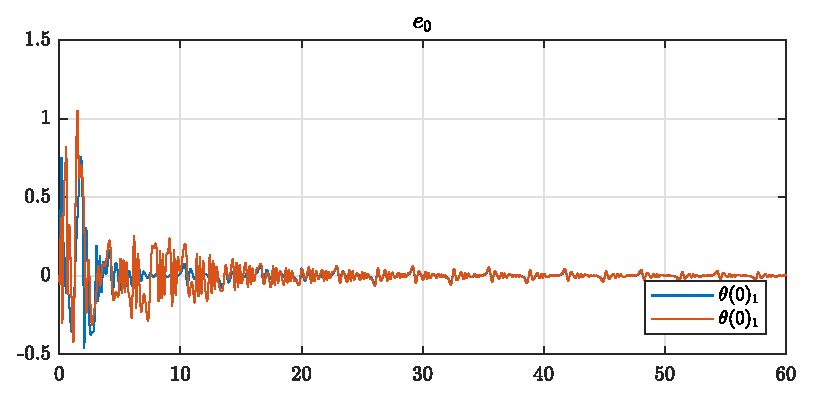
\includegraphics[width=12cm]{figs/e0/sim0_theta0.eps} 
\end{figure}

\begin{figure}[H]
  \centering
  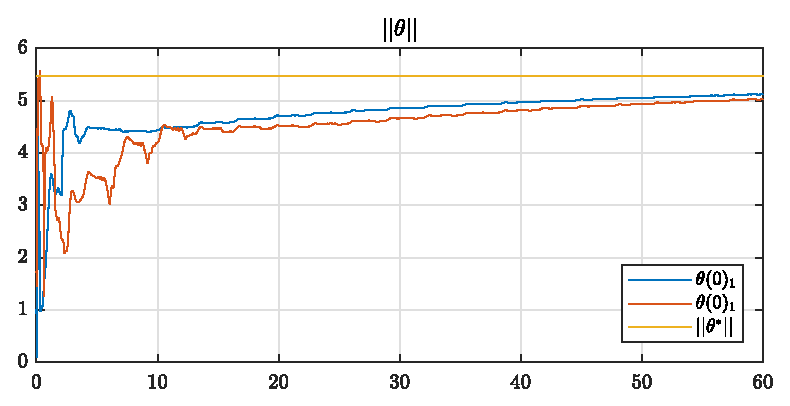
\includegraphics[width=12cm]{figs/modtheta/sim0_theta0.eps} 
\end{figure}

\begin{figure}[H]
  \centering
  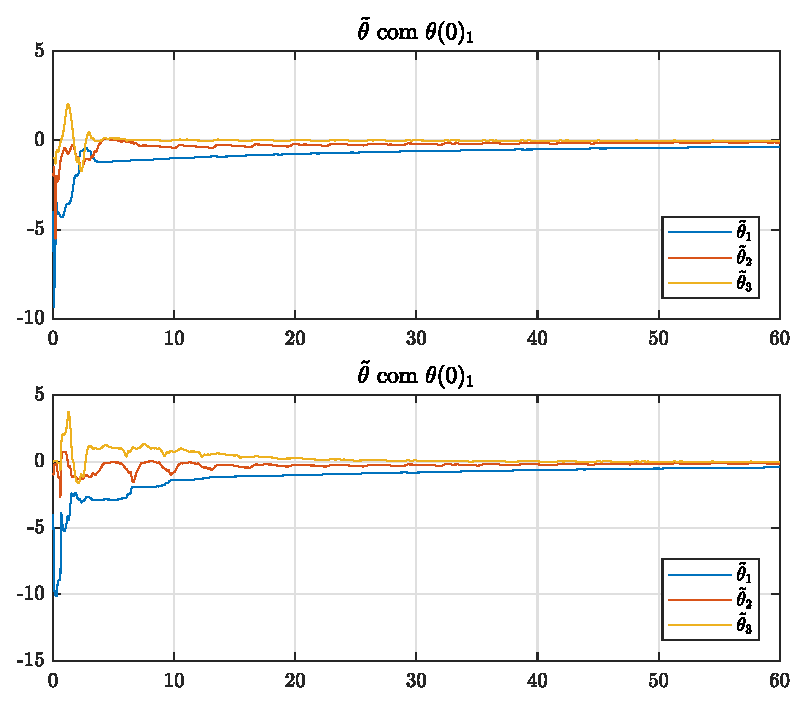
\includegraphics[width=12cm]{figs/tiltheta/sim0_theta0.eps} 
\end{figure}

\begin{figure}[H]
  \centering
  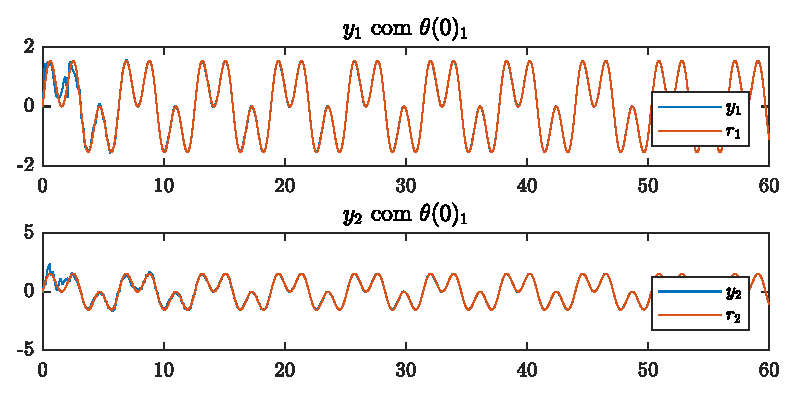
\includegraphics[width=12cm]{figs/y/sim0_theta0.eps} 
\end{figure}

\textbf{\underline{Simula��o 1.2}: $y(0)$}
%
\begin{align*}
  y &= \frac{5}{s^2+2s+1}u\,,  &  \theta(0) &= 0 \,,
  & y(0) &=  \HI{0} \, \textrm{e} \, \HI{5} \,, & \Gamma &= 10 \,
  \textbf{I}_3\,, \\ y_r &= \textrm{sin}(t) + \textrm{sin}(3t) \, .
\end{align*}

\begin{figure}[H]
  \centering
  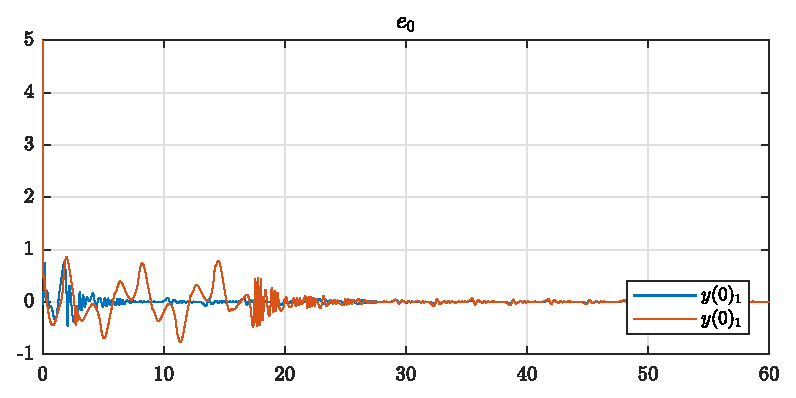
\includegraphics[width=12cm]{figs/e0/sim0_y0.eps} 
\end{figure}

\begin{figure}[H]
  \centering
  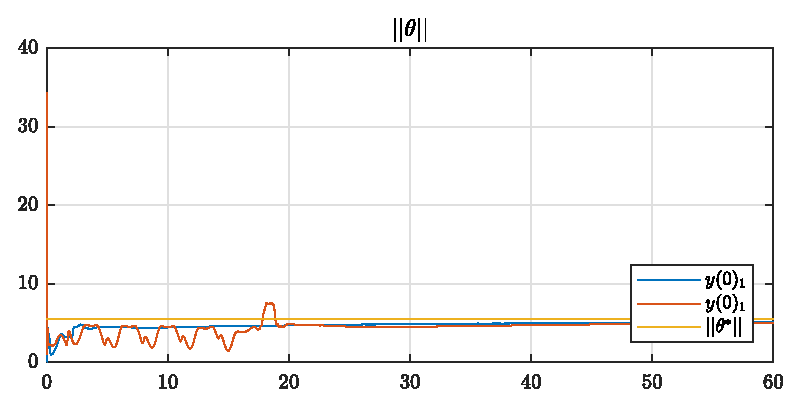
\includegraphics[width=12cm]{figs/modtheta/sim0_y0.eps} 
\end{figure}

\begin{figure}[H]
  \centering
  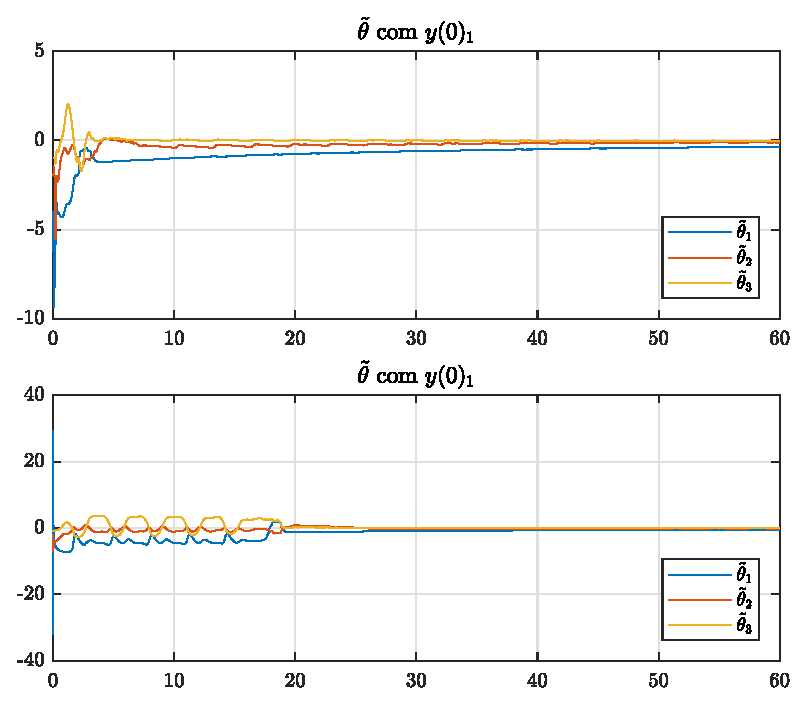
\includegraphics[width=12cm]{figs/tiltheta/sim0_y0.eps} 
\end{figure}

\begin{figure}[H]
  \centering
  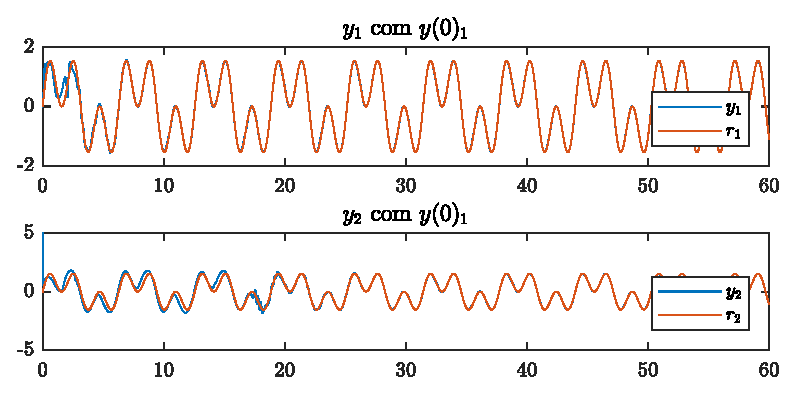
\includegraphics[width=12cm]{figs/y/sim0_y0.eps} 
\end{figure}

\subsection{Simula��o \#2}

Verificamos o comportamento do sistema para varia��es no par�metro de adapta��o
$\Gamma$.

\bigskip

\begin{align*}
  y &= \frac{5}{s^2+2s+1}u\,,  &  \theta(0) &= 0 \,,
  & y(0) &=  0 \,, & \Gamma &= \HI{1} \, \textrm{e} \, \HI{10} \,
  \textbf{I}_3\,, \\ y_r &= \textrm{sin}(t) + \textrm{sin}(3t) \, .
\end{align*}

\begin{figure}[H]
  \centering
  \includegraphics[width=12cm]{figs/e0/sim0_gamma10gamma1.eps} 
\end{figure}

\begin{figure}[H]
  \centering
  \includegraphics[width=12cm]{figs/modtheta/sim0_gamma10gamma1.eps} 
\end{figure}

\begin{figure}[H]
  \centering
  \includegraphics[width=12cm]{figs/tiltheta/sim0_gamma10gamma1.eps} 
\end{figure}

\begin{figure}[H]
  \centering
  \includegraphics[width=12cm]{figs/y/sim0_gamma10gamma1.eps} 
\end{figure}

\subsection{Simula��o \#3}

Verificamos o comportamento do sistema para varia��es na planta e modelo.

\bigskip

\textbf{\underline{Simula��o 3.1}: planta}
%
\begin{align*}
  y &= \frac{5}{s^2+2s+1}u\, \textrm{e} \, \frac{5}{s^2-2s+1}u,  &  \theta(0) &=
  0 \,, & y(0) &=  0 \,, & \Gamma &= 10 \,
  \textbf{I}_3\,, \\ y_r &= \textrm{sin}(t) + \textrm{sin}(3t) \, .
\end{align*}

\begin{figure}[H]
  \centering
  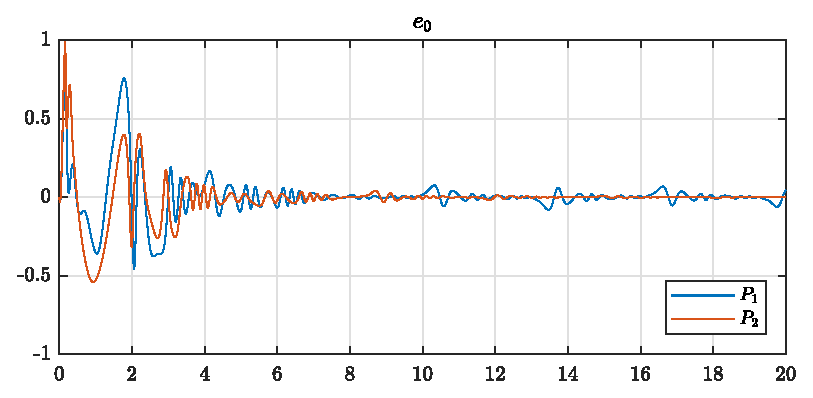
\includegraphics[width=12cm]{figs/e0/sim0_P1P2.eps} 
\end{figure}

\begin{figure}[H]
  \centering
  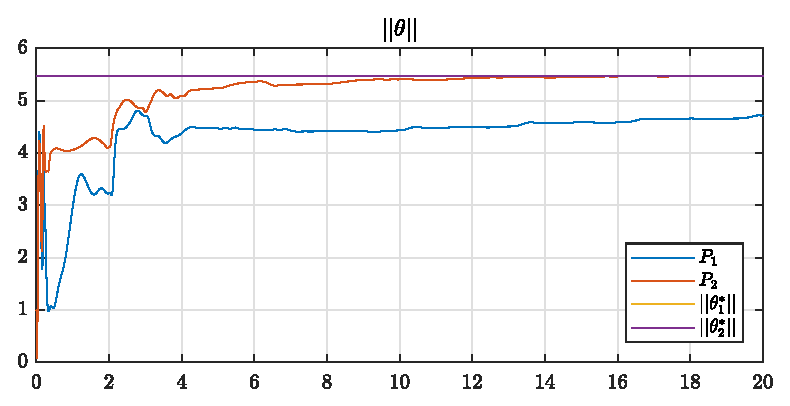
\includegraphics[width=12cm]{figs/modtheta/sim0_P1P2.eps} 
\end{figure}

\begin{figure}[H]
  \centering
  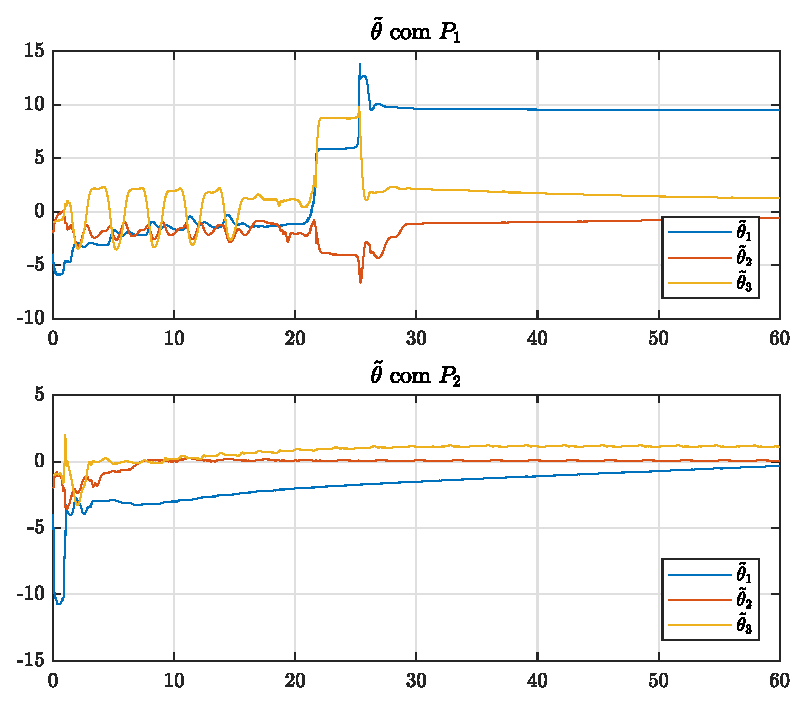
\includegraphics[width=12cm]{figs/tiltheta/sim0_P1P2.eps} 
\end{figure}

\begin{figure}[H]
  \centering
  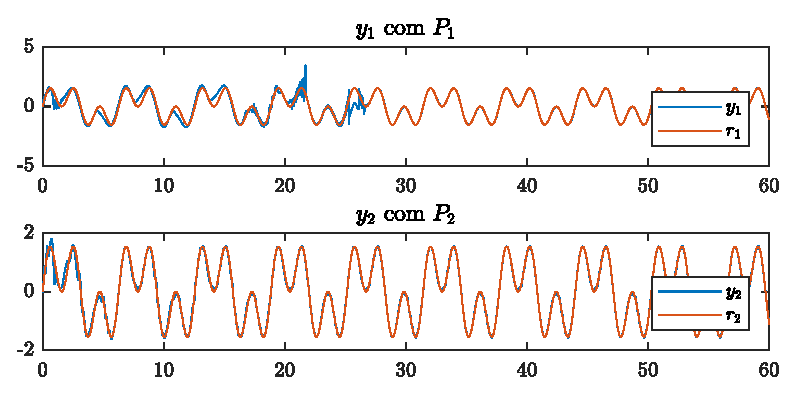
\includegraphics[width=12cm]{figs/y/sim0_P1P2.eps} 
\end{figure}

\textbf{\underline{Simula��o 3.2}: modelo}
%
\begin{align*}
  y &= \frac{5}{s^2+2s+1}u\, &  \theta(0) &=
  0 \,, & y(0) &=  0 \,, & \Gamma &= 10 \,
  \textbf{I}_3\,, \\ y_r &= \textrm{sin}(t) + \textrm{sin}(3t) \, \textrm{e} \,
  \textrm{sin}(t) + \textrm{2sin}(5t) .
\end{align*}
 
\begin{figure}[H]
  \centering
  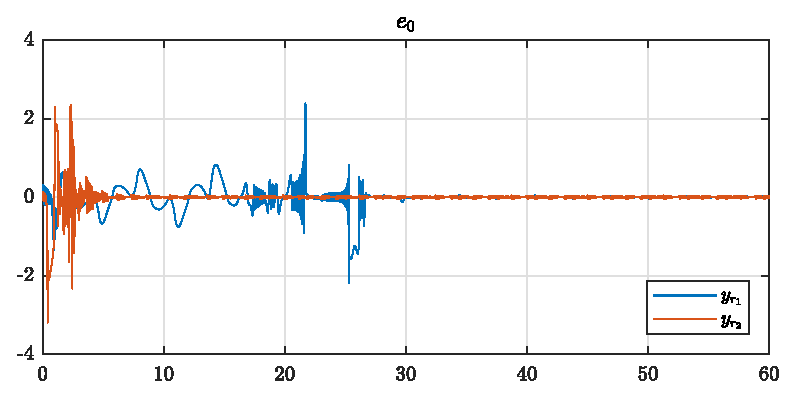
\includegraphics[width=12cm]{figs/e0/sim0_yr1yr2.eps} 
\end{figure}

\begin{figure}[H]
  \centering
  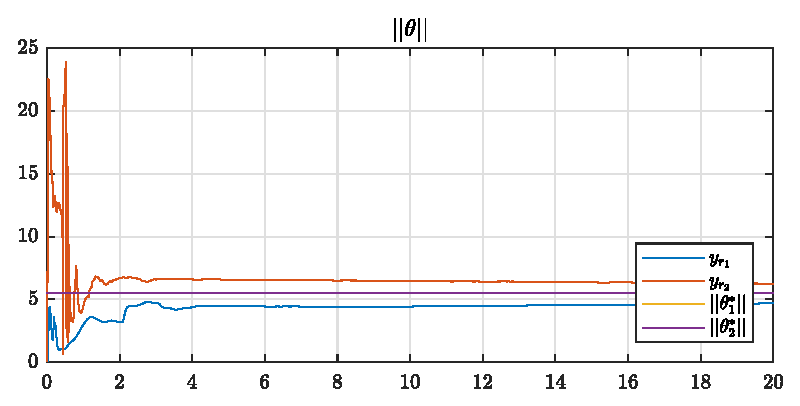
\includegraphics[width=12cm]{figs/modtheta/sim0_yr1yr2.eps} 
\end{figure}

\begin{figure}[H]
  \centering
  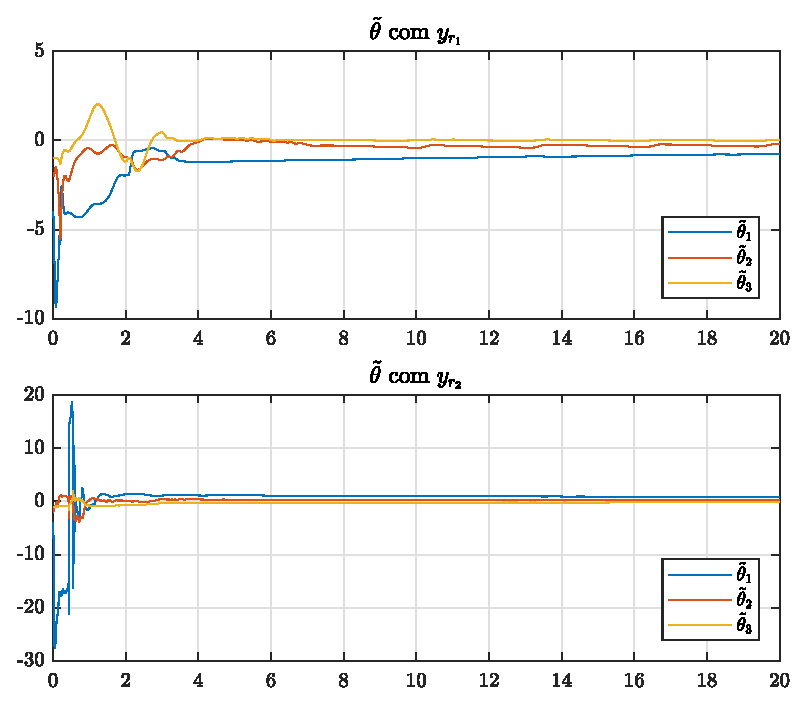
\includegraphics[width=12cm]{figs/tiltheta/sim0_yr1yr2.eps} 
\end{figure}

\begin{figure}[H]
  \centering
  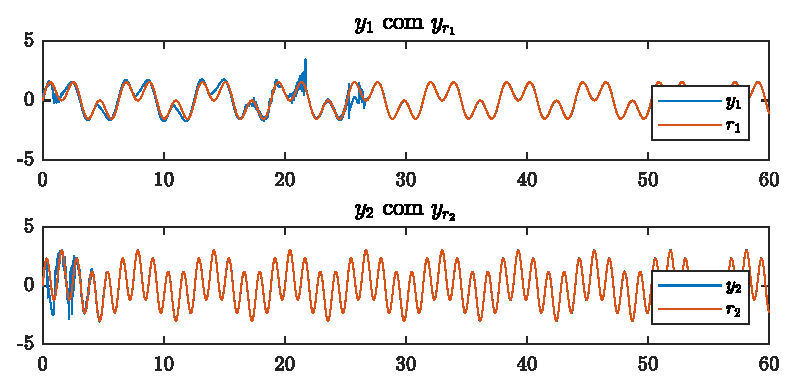
\includegraphics[width=12cm]{figs/y/sim0_yr1yr2.eps} 
\end{figure} \newpage
%---------------------------------------------------------------------
\section{Discuss�o}

As conclus�es deste trabalho s�o bastante semelhantes ao Trabalho 7, que trata do m�todo Backstepping para observador de ordem completa. Iremos repetir aqui a mesma discuss�o encontrada no relat�rio do trabalho 7 por conveni�ncia e ent�o faremos um breve comparativo entre o desempenho dos observadores.

A \textbf{simula��o \#1} mostra o comportamento do sistema para varia��es nas
condi��es iniciais. A rapidez da converg�ncia depende de qu�o pr�ximo os par�metros estimados est�o dos par�metros reais. A simula��o mostrou um comportamento semelhante para ambos os casos. Quando deslocamos o $y(0)$, os sistemas tamb�m
apresentam comportamento semelhante, pois a vari�vel de controle $u$ � alterada
e n�o apresenta satura��o, compensando a condi��o inicial.

A \textbf{simula��o \#2} mostra o comportamento do sistema para varia��es na
planta. Escolhemos plantas inst�veis e est�veis. Podemos observar que, em ambos
os casos, o sinal de controle foi capaz de corrigir o erro, sem muitas
dificuldades. O comportamento dos sistemas � semelhante e para a planta 2, houve at� converg�ncia dos par�metros $\theta$.

Na \textbf{simula��o \#3}, foram testadas duas refer�ncias $y_r$ distintas, que tamb�m podem ser entendidas como a resposta de um modelo de refer�ncia $P_m(s)$ a uma refer�ncia $r(t)$. A altera��o no sinal de refer�ncia mostrou que sinais mais complexos, com frequ�ncias mais altas e maiores amplitudes, demoram um pouco mais para convergir.

Finalmente, a \textbf{simula��o \#4} mostra o comportamento do sistema para varia��es no
ganho de adapta��o $\Gamma$. Podemos verificar converg�ncia mais r�pida quando o
$\Gamma$ � maior, por�m tamb�m observamos maiores oscila��es e picos de erro.

Como utilizamos os mesmos par�metros entre as simula��es do Backstepping com observador de ordem completa e de ordem reduzida, podemos comparar o desempenho dos dois observadores. No geral, nota-se um desempenho superior do observador de ordem completa: menor amplitude de oscila��es residuais, tempo de converg�ncia menor e picos de transit�rio menores. No entanto, o esfor�o computacional do observador completo � maior que o observador de ordem reduzida. 
%---------------------------------------------------------------------
%\bibliographystyle{agsm}
%\bibliography{bib,coe736}

%---------------------------------------------------------------------
\end{document}
